\documentclass{article}
\usepackage{kotex}
\usepackage{amssymb}
\usepackage{amsmath}
\usepackage{setspace}
\usepackage{graphicx}
\usepackage{booktabs}
\usepackage{subfigure}
\begin{document}
\setstretch{1.6}

\title{머신 러닝을 통한 신재생에너지 예측 최적화}
\author{18009 고도형}
\maketitle

\section{서론}
고객들의 필요에 따라 적절한 양의 에너지를 공급하기 위해 전력을 공급하는 회사들은 발전소의 생산율을 조절하고 다른 회사로부터 전력을 수입해서 수요를 충족시켜 왔다. 그러나 갈수록 필요한 전기에너지의 양이 증가하면서 수요가 전체 발전소의 생산량을 합한 것보다 큰 상황이 발생하는 것에 대비해 전력 시장에서 공급뿐만 아니라 수요를 조절하는 것도 필요해졌다. 그리하여 현재 전력 공급량에 맞추어 전기 사용자가 자신의 사용량을 변화시키는 수요 반응(DP; Demand Response)의 개념이 등장했다. 수요 반응은 현재 시장에서 제공 가능한 에너지의 양에 따른 인센티브를 제공하여 그에 따라 자연스럽게 소비자가 스스로의 전기 사용에 변화를 만드는 것을 말한다. 그리고 효율적인 에너지 사용을 위하여 도입된 스마트 그리드 시스템은 에너지를 절감하고 효율적으로 사용하기 위해 전력 시장에서 소비자의 능동적이고 자발적인 수요반응을 활용한다. 그리고 이를 위해 전력 수요를 상시 모니터링하며 수요의 증감에 따라 필요한 발전소의 발전량을 조절한다. 다행히 가정이나 공장의 전력 수요는 누적된 데이터를 통해 어렵지 않게 예측할 수 있고 전력을 수급하기 위한 발전소의 선택과 전력의 공급 시기를 정확히 만족시킬 수 있다. \newline
그런데 에너지의 초과수요를 방지하고 소비자로부터 수요 반응을 이끌어내기 위해서는 전력 수요뿐만 아니라 특정 시점에서의 한계 공급량이 어느 정도인지 미리 파악할 필요가 있다. 일반적인 화력 발전이나 원자력 발전의 경우에는 시간에 따른 발전량의 기복이 크지 않아 한계 공급량을 어렵지 않게 파악할 수 있으나 대부분의 신재생에너지는 기상 상황에 따라 발전량의 차이가 커 예측이 불가능하고 관리하기가 쉽지 않다. 이러한 신재생에너지의 발전량은 기상 파라미터 값과 깊은 연관성을 가지는 만큼 정확한 예측을 위해 주로 기상 데이터를 이용한 기계적 모델이 채택되고 있다.

\section{선행 연구}
Emil Isaksson과 Mikael Karpe Conde은 논문 Solar Power Forecasting with Machine Learning Techniques에서 머신 러닝 기반의 태양광 발전량 예측 모델을 설계하였다. 이 모델은 지도학습 알고리즘 중 하나인 K-최근접 이웃 방법을 활용하여 높은 정확도로 한계 공급량을 예측하였다. 연구진은 과거의 각종 기상 데이터들을 바탕으로 해당 환경 아래에서 실제 발전량과 근접하게 예측할 수 있는 모델을 훈련시키고 기상 예보 데이터를 접목시켜 전력 생산량을 예측하였다.

\section{KNN: K-Nearest Neighbor}
연구에 사용된 KNN 알고리즘은 K-최근접 이웃(K-nearest neighbor)이라 불리는 지도학습 알고리즘이다. 본래 데이터를 여러 개의 클래스로 구별하는 분류(Classification) 문제에 적합하게 설계되었으나 논문에서는 이를 회귀 문제에 적용하였다. /newline
기본적으로 주어진 데이터 $X$로부터 특정 클래스에 속한 주변 데이터의 위치를 고려하여 가장 높은 확률을 가지는 클래스로 $Y$의 값을 추정한다. 즉, 다음과 같은 과정을 거친다. 우선, 어떠한 테스트 데이터 $x_0$와 클래스 $j$가 존재할 때, $x_0$로부터 가장 가까운 유클리드 거리(Euclidean distance)를 가지는 $K$개의 데이터들의 순열 $N_0$을 구한다.
\begin{equation}
dist(x_0, K)=\sqrt{\sum_{i=1}^{K}(x_0-X_i)^2}
\end{equation}
다음으로, 추정값 $Y=j$를 만족할 확률을 $x_0$로부터 가장 가까운 $K$개의 데이터 중 클래스 $j$에 속하는 것의 개수와 전체 $K$의 값을 바탕으로 아래와 같이 정의한다.
\begin{equation}
Pr(Y=j | X=x_0)=\frac{1}{K}\sum_{i \in N_0}I(y_i=j)
\end{equation}
최종적으로 $x_0$는 가장 높은 확률을 가진 클래스 $j$에 배정하는 것이 KNN 알고리즘의 동작 원리이다. 테스트 데이터를 기준으로 고려할 데이터의 개수를 결정하는 $K$의 값은 알고리즘에서 중요한 위치를 차지하는데 이는 이후 교차검증(Cross-Validation)의 방법을 통해 해결하였다.
앞서 언급하였던 분류 문제에서의 방법과 거의 동일하지만 회귀 문제에 적용되는 알고리즘은 데이터의 추정값을 이웃한 데이터 값들의 평균으로 정의하여 동작한다는 차이가 있다. 즉, 테스트 데이터의 추정값은 다음과 같이 $K$번째로 가까운 주변 데이터들의 집합의 평균값으로 정의된다.
\begin{equation}
\hat{Y}=\frac{1}{K}\sum_{i \in N_0}y_i
\end{equation}

\section{교차검증: K-Fold Cross Validation}
검증 데이터 집합(Validation Dataset)은 훈련 데이터 집합(Training data set)으로 모델링을 시도할 때, 학습 상태를 점검하고 하이퍼파라미터를 조절할 수 있도록 하는 데이터 집합이다. 이러한 검증 데이터 집합은 일반적으로 훈련 데이터 집합에서 $n:m$ 비율로 나누어 사용하는데 이 연구에서는 하이퍼파라미터 중 하나인 KNN 알고리즘의 $K$값을 탐색할 때 적용되었다. \newline

\begin{figure}[h]
\centering
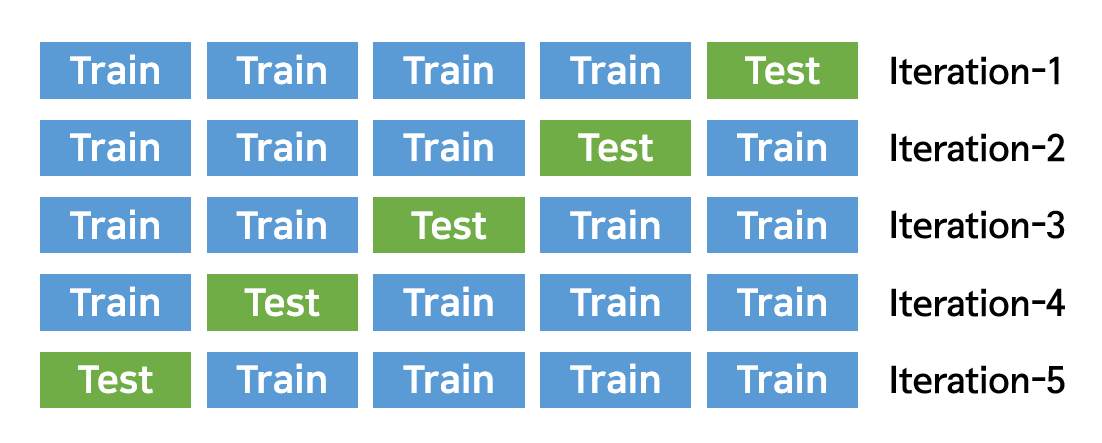
\includegraphics[scale=0.5]{./fig/Figure_1.png}
\caption{Process of Cross Validation}
\label{fig_1}
\end{figure}

아래 Figure 1에서 볼 수 있듯 총 5번의 훈련을 진행한다고 할 때, 각각의 훈련 단계(iteration)에서 훈련 데이터 집합을 5개의 부분집합으로 쪼개고 그 중 하나를 검증 데이터 집합으로 설정하여 알고리즘의 학습 상태를 점검하는 것을 알 수 있다. 연구에서 사용된 K-Fold Cross Validation 방법은 1개의 훈련 데이터 집합을 $K$개로 나누어 그 중 1개를 검증 데이터 집합으로, 나머지 $K-1$개를 훈련 데이터 집합으로 하여 모델을 학습시키는 것을 의미한다.

\section{데이터}
해당 연구에서는 모델을 훈련시키기 위해 다양한 형태의 기상 데이터들을 사용하였다. 연구가 스웨덴의 5개 지역에 대해 진행된 만큼 데이터 또한 각각의 지역에서 동일한 조건 아래 측정되었다. 우선, 2~3년에 걸쳐 15분간격으로 측정한 파워 데이터는 고정된 태양광 PV 패널의 하루 기준 시간당 발전량을 kWh로 측정된 것이다. 이 데이터는 특정 기상 조건에서 실제 발전량을 나타내는 지표로 사용되었으며 모델의 추정값과 대조하여 그 오차를 줄이는 데 실질적으로 사용되었다.

\begin{figure}[h]
\centering
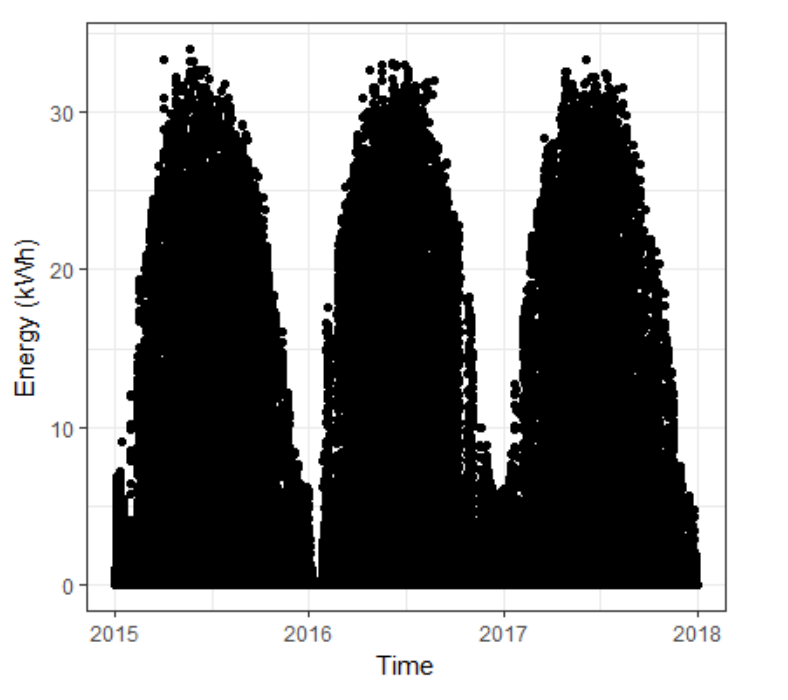
\includegraphics[scale=0.20]{./fig/Figure_2.png}
\caption{Energy Output for one of the 5 sites}
\label{fig_2}
\end{figure}

다음으로, 수치적 기상 예측 데이터(Numerical Weather Prediction Data)이다. Meteomatics의 API로부터 5개 지역의 2~3년 동안의 다양한 기상학적 변수들의 값을 얻었다. 이 데이터는 알고리즘의 실질적인 파라미터로 설정되어 적절한 추정 모델을 구성하는데 기여하였다. 자세한 정보는 다음 표를 참조하라. \newline
\begin{table}[h]
    \begin{tabular}{@{}|c|c|c|@{}}
    \toprule
    \textbf{변수명}                & \textbf{NWP 데이터}                      & \textbf{단위} \\ \midrule
    total\_cloud\_cover : p     & 구름의 양                                 & \%          \\
    wind\_speed\_10m : ms       & 지상 10m 높이의 풍속                         & m/s         \\
    wind\_dir\_10m : d          & 지상 10m 높이의 풍향                         & m/s         \\
    t\_2m : C                   & 지상 2m 높이의 기온                          & C           \\
    clear\_sky\_rad : W         & Clear Sky Radiation                   & $W/m^2$     \\
    sfc\_pressure : hPa         & 기압                                    & hPa         \\
    diffuse\_rad : W            & 산란복사의 순간 Flux                         & $W/m^2$     \\
    global\_rad : W             & 전천복사의 순간 Flux                         & $W/m^2$     \\
    direct\_rad : W             & 직달 태양 복사의 순간 Flux                     & $W/m^2$     \\
    effective\_cloud\_cover : p & Effective Cloud Cover                 & \%          \\
    high\_cloud\_cover : p      & High Cloud Cover                      & \%          \\
    medium\_cloud\_cover : p    & Low Cloud Cover                       & \%          \\
    precip\_1h : mm             & 누적 강수량 (1시간)                          & mm          \\
    fresh\_snow\_1h : cm        & 누적 적설량 (1시간)                          & cm          \\
    global\_rad\_1h : J         & 누적 전천복사량 (1시간)                        & J           \\
    direct\_rad\_1h : J         & 누적 직달 태양복사량 (1시간)                     & J           \\
    diffuse\_rad\_1h : J        & 누적 산란복사량 (1시간)                        & J           \\
    cape : Jkg                  & Convective Available Potential Energy & J/kg of air \\
    relative\_humidity\_2m : p  & 지상 2m 지점의 상대 습도                       & \%          \\ \bottomrule
\end{tabular}
\caption{\label{tab:table_1}NWPs from Meteomatics}
\end{table}

\begin{figure}[!h]
\centering
\subfigure[A cloudy day]{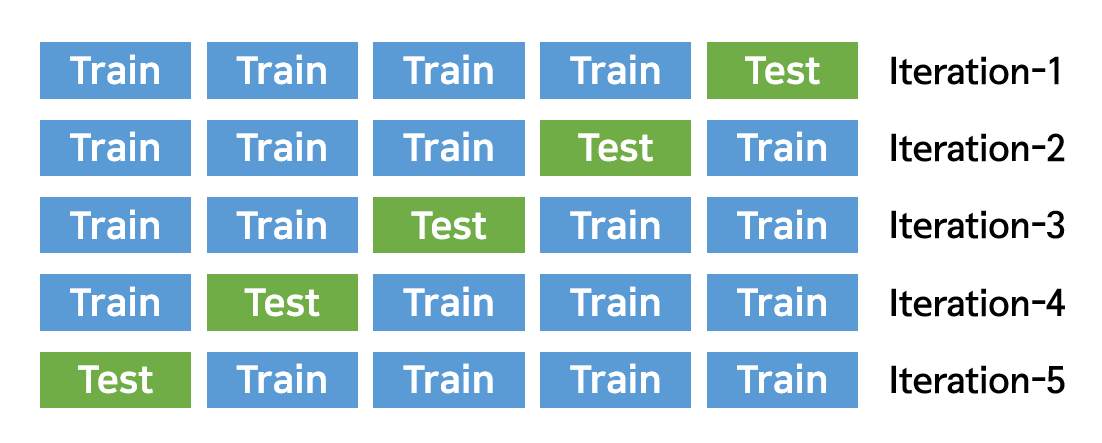
\includegraphics[width=0.45\textwidth]{./fig/Figure_3.PNG}\hfill}
\subfigure[A sunny day]{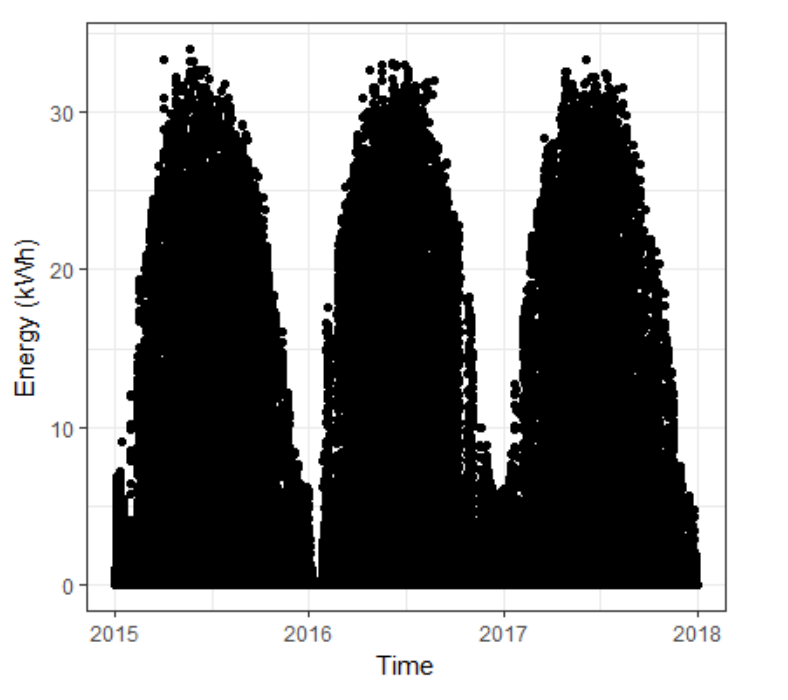
\includegraphics[width=0.45\textwidth]{./fig/Figure_4.PNG}\hfill}
\caption{Correlation between NWP Data and Energy output}
\label{fig_3}
\end{figure}

Figure 3은 NWP 데이터 중 하나인 구름의 양(Total Cloud Cover)과 해당 조건에서의 서로 다른 두 태양광 PV 패널 사이의 발전량의 차이를 나타낸 그래프이다. 이처럼 Table 1의 다양한 변수를 파라미터로 하는 머신 러닝 모델을 구현함으로서 파라미터에 따른 예상 에너지 생산량을 최적화할 수 있다.

\section{머신 러닝 모델}
추정값과 실제값 사이의 차이를 측정하기 위해 연구진은 아래의 평균 제곱근 오차(RMSE: Root Mean Squared Error)를 적용하였다.
\begin{equation}
RMSE=\sqrt{\frac{\sum_{i=1}^{n}(Y_i-\hat{Y_i})^2}{n}}
\end{equation}
$Y_i$는 실제 데이터의 값을, $\hat{Y_i}$는 예측한 데이터의 값을 나타낸다.
그리고 이를 바탕으로 다음과 같은 기상 데이터에 따른 발전량 예측 모델을 설계하였다. 다음은 모델의 의사코드를 표현한 것이다.

\begin{figure}[h]
\centering
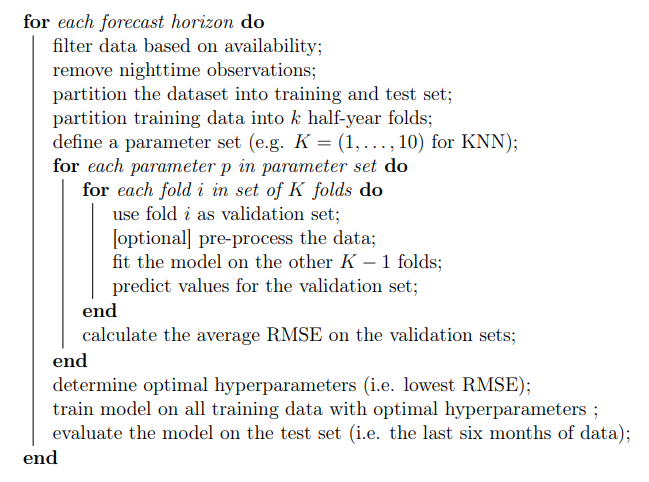
\includegraphics[scale=0.70]{./fig/Figure_5.png}
\caption{Pseudocode for Algorithm}
\label{fig_4}
\end{figure}



\end{document}